\section{State Space Description}

\subsection{State Space Description}

\begin{minipage}{10cm}
    \begin{align*}
        \dot{\underline{x}}(t) &= A \underline{x}(t) + B \underline{u}(t) \\
        \underline{y}(t) &= C \underline{x}(t) + D\underline{u}(t)
    \end{align*}
    with the number of state variables $n$, the number of input signals $M$ and the number of output signals $P$.
\end{minipage}
\hspace{0.5cm}
\begin{minipage}{8cm}
    \centering
    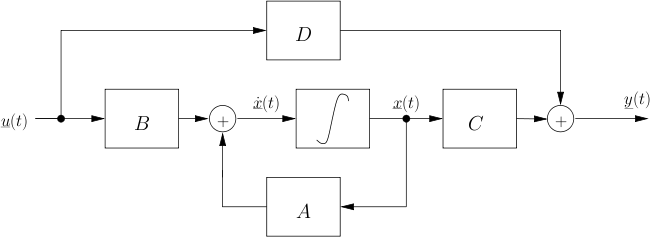
\includegraphics[width=\linewidth]{./bilder/zrd-schema.png}
\end{minipage}

\begin{tabularx}{\linewidth}{llll}
    $A$: & $n \times n$ & system matrix & describes the dynamics of the system. \\
    $B$: & $n \times M$ & input matrix & describes how the input influences state variables. \\
    $C$: & $P \times n$ & output matrix & describes how the output depends on state variables. \\
    $D$: & $P \times M$ & feed-through matrix & describes direct coupling between $u$ and $y$. 
\end{tabularx}

\subsection{Input-Output Description}
For a MIMO system with $M$ inputs and $P$ outputs, $G(s)$ is a $P \times M$ matrix of transfer functions.
\begin{align*}
    G(s) &= \frac{Y(s)}{U(s)} = \frac{b_{m} s^{m} + b_{m-1} s^{m-1} +\cdots+b_{1} s 
    + b_{0}}{s^{n} + a_{n-1} s^{n-1} + \cdots + a_{1} s + a_{0}} \\
    &= C (sI-A)^{-1} B + D
\end{align*}
The inversion of $G(s)$ to find a state space description is not unique.

\subsubsection{Controllable Canonical Form}
The controllable canonical form uses a slightly different I/O-description:
\[
    G(s) = \frac{Y(s)}{U(s)} = \frac{b_{n-1} s^{n-1} + b_{n-2} s^{n-2} +\cdots+b_{1} s 
    + b_{0}}{s^{n} + a_{n-1} s^{n-1} + \cdots + a_{1} s + a_{0}} + d
\]
which corresponds to
\begin{align*}
    A_c &= \begin{bmatrix}
        0 & 1 & 0 & \dots \\
        \vdots & \ddots & \ddots & \vdots \\
        0 & \dots & 0 & 1 \\
        -a_0 & -a_1 & \dots & -a_{n-1}
    \end{bmatrix} &
    B_c &= \begin{bmatrix}
        0 \\ \vdots \\ 0 \\ 1
    \end{bmatrix} \\
    C_c &= \begin{bmatrix}
        b_0 & b_1 & \dots & b_{n-1} 
    \end{bmatrix} &
    D_c &= d
\end{align*}

\subsubsection{Observable Canonical Form}
\begin{align*}
    A_o &= \begin{bmatrix}
        0 & 0 & \dots & -a_0 \\
        1 & 0 & \dots & -a_1 \\
        \vdots & \ddots & \ddots & \vdots \\
        0 & \dots & 1 & -a_{n-1}
    \end{bmatrix} &
    B_o &= \begin{bmatrix}
        b_0 \\ b_1 \\ \vdots \\ b_{n-1}
    \end{bmatrix} \\
    C_o &= \begin{bmatrix}
        0 & \dots & 0 & 1
    \end{bmatrix} & 
    D_o &= d
\end{align*}

\subsection{Similarity Transform}
The state space description is not unique and depends on the selection
of the state variables in $x$.
This allows for any \emph{similarity} transformation
\[
    \tilde{x}(t) = T x(t)
\]
which leads to
\begin{align*}
    \tilde{A} &= T A T^{-1} &
    \tilde{B} &= T B & 
    \tilde{C} &= C T^{-1} &
    \tilde{D} &= D
\end{align*}

\subsection{Minimal State Space Realization}
A minimal state space realization contains the \emph{minimal} number of integrators.
A transfer function $G(s)$ of order $n$ results in a state-space of order $n$, i.e.
with $n$ integrators.

\paragraph{SISO systems}The fraction is fully reduced, i.e. contains no common poles and zeros.

\paragraph{MIMO systems}Not easily possible. Try to find realization with minimum number of integrators.

\subsection{Controllability and Observability}
A state space describtion is controllable \emph{and} observable if (and only if) it is minimal.

\paragraph{Controllability}A pair $(A,B)$ is controllable if an input $u(t)$ can transfer any
initial state $x(0)$ into another state $x(T)$ in finite time $T$.
It is controllable if the eigenvalues of $A-BK$ can be placed arbitrarily, thus$P_c$ has full rank:
\[
    \rank(P_c) = \rank(
        \begin{bmatrix}
            B & AB & A^2B & \dots & A^{n-1}B
        \end{bmatrix}
    ) = n
\]

\paragraph{Observability}A pair $(A,C)$ is observable if the initial state $x(0)$ can
be determined from the observation of $y(t)$ given the control $u(t)$ within finite time $T$.
It is observable, if the eigenvalues of $A-HC$ can be placed arbitrarily, thus $P_o$ has full rank:
\[
    \rank(P_o) = \rank(
        \begin{bmatrix}
            C \\ C A \\ \vdots \\ C^{n-1}
        \end{bmatrix}
    ) = n
\]

\subsection{Stability}
A system in I/O-describtion is (asymptotically) stable if all the poles have a negative real part.
In that cae, the impulse response $g(t)$ converges to $0$.
In state space, all eigenvalues of $A$ must have a negative real part.
